\section{Extended Pillar Catalogs}
\label{supp:sec:extended-pillars}

This supplement preserves the extended system catalogs, secondary variants, and benchmark evidence supporting the four pillar chapters in the main article. The organization follows those chapters, while every label is local to the supplement.

\subsection{Extended Catalog: Language as Grounding Signal}
\label{supp:sec:grounding}

\begin{figure}[t]
    \centering
    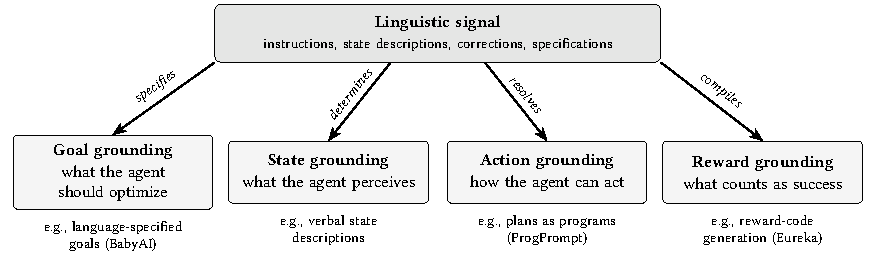
\includegraphics[width=\linewidth]{paper_images/generated/grounding_mapping.pdf}
    \Description{A linguistic signal branches to goal, state, action, and reward grounding. Each branch states the decision-problem role and one example.}
    \caption{Grounding signals map verbal input onto four decision-problem components at specification time.}
    \label{supp:fig:grounding-mapping}
\end{figure}

\subsubsection{Historical lineage and goal grounding}
\label{supp:subsec:grounding-goals}

Grounding language in sequential decision making predates large language models. Mapping instructions to actions was formulated as a reinforcement-learning problem before pretrained interpreters existed \citep{branavan2009reinforcement,misra2017mapping}, policy sketches used linguistic annotations to decompose multitask learning \citep{andreas2017modular}, and agents acquired grounded word meanings in simulated three-dimensional worlds \citep{hermann2017grounded}. The earlier literature separated language-conditional from language-assisted reinforcement learning \citep{luketina2019survey}, while language-conditioned imitation extended grounding to robot control \citep{lynch2021language}. Current systems inherit much of the interpreter from pretraining and use it to compile specifications.

Goal grounding requires parsing instructions into objects, relations, and target conditions \citep{chaplot2018gated}, filtering candidate plans by executability \citep{ahn2022can,driess2023palm}, and decomposing goals into verifiable subgoals. Secondary variants include multi-agent coordination \citep{zhang2025towards}, hierarchical goal decomposition through offline reinforcement learning \citep{hu2025divide}, and policies trained directly from language specifications \citep{li2026ground}. BabyAI isolates compositional generalization in gridworlds \citep{chevalier2018babyai}; current models still show incomplete coverage under compositional constraints \citep{sakai2025revisiting}, while compositional policy representations improve sample efficiency on unseen combinations \citep{cohen2025compositional}.

\subsubsection{State and action grounding}
\label{supp:subsec:grounding-state-action}

Verbal state descriptions are native to text environments \citep{yao2020keep,cote2018textworld}, but they also arise whenever visual or physical state is summarized into language. ALFWorld shows transfer from verbal descriptions to embodied three-dimensional settings \citep{shridhar2020alfworld}. Later work adds closed-loop verbal state feedback for robot planning \citep{bhat2024grounding} and scene-graph-structured context \citep{huang2025escacontextualizingembodiedagents}. These systems expose a recurring limitation: verbalization can silently violate the Markov property when omitted details carry decision-relevant history.

Action grounding ranges from corrective planning to compilation into programs. Inner Monologue feeds verbalized success detection and scene description back into planning \citep{huang2022inner}, while concise corrective utterances can amend a local error without discarding the rest of a plan \citep{sharma2022correcting}. ProgPrompt represents available actions and objects in program-like form \citep{singh2022progprompt}; VoxPoser converts language into three-dimensional value maps consumed by a motion planner \citep{huang2023voxposer}. Secondary systems combine visual cues with grounded replanning \citep{kim2025multi}, detect failures through constraint-aware visual programs \citep{zhou2025code}, span physical, logical, and semantic corrections across control levels \citep{joublin2024copal}, or join language reasoning with feasibility checking in task-and-motion planning \citep{zhang2025llm}. RT-H inserts fine-grained language motions between task and actuation so human corrections arrive in the policy's own intermediate action space \citep{belkhale2024rth}.

\subsubsection{Reward-grounding systems and evidence}
\label{supp:subsec:grounding-reward}

Language-to-reward methods differ in how directly text specifies the executable objective. Eureka evolves generated reward programs and uses training statistics as textual reflection \citep{ma2024eureka}; Text2Reward generates dense, human-refinable code \citep{xie2024text2reward}. DrEureka extends generation to domain-randomization settings needed for simulation-to-real transfer \citep{ma2024dreureka}; CARD refines reward code from trajectory feedback without retraining a policy at every iteration \citep{sun2025large}; PROF adapts the mechanism to offline settings \citep{sun2025prof}; and reward functions can be generated from video demonstrations \citep{zeng2024video2reward}.

Structured alternatives let language select reward parameters rather than write unrestricted code. Language to Rewards maps instructions and corrections to parameters consumed by a real-time optimizer and outperforms a primitive-skill baseline based on Code as Policies \citep{yu2023language,liang2022code}. When no compilable state is exposed, a learned judge grounds the objective in observations. RL-VLM-F uses vision-language preferences over image pairs \citep{wang2024rlvlmf}, while purpose-trained visual reward models aim for broader reward provision \citep{lee2026roboreward,schroeder2026soler1}.

Reward-grounding errors are specification failures rather than ordinary estimation noise. A syntactically valid reward can encode the wrong objective and then be optimized exactly. Iterative reflection searches reward-function space, and related methods use language to redistribute sparse rewards. LaRe constructs symbolic latent-reward evaluators from language \citep{qu2024latent}; Agent-RLVR instead densifies a sparse verifier with teacher-style guidance on software-engineering tasks \citep{da2025agentrlvr}. Controlled evidence also shows that diverse and informative feedback improves transfer and adaptation \citep{xi2024teaching}. These results motivate explicit checks for executability, compositionality, and fidelity before downstream policy performance is interpreted.

\subsection{Extended Catalog: Language as Deliberative Feedback}
\label{supp:sec:deliberative}

\begin{figure}[!t]
    \centering
    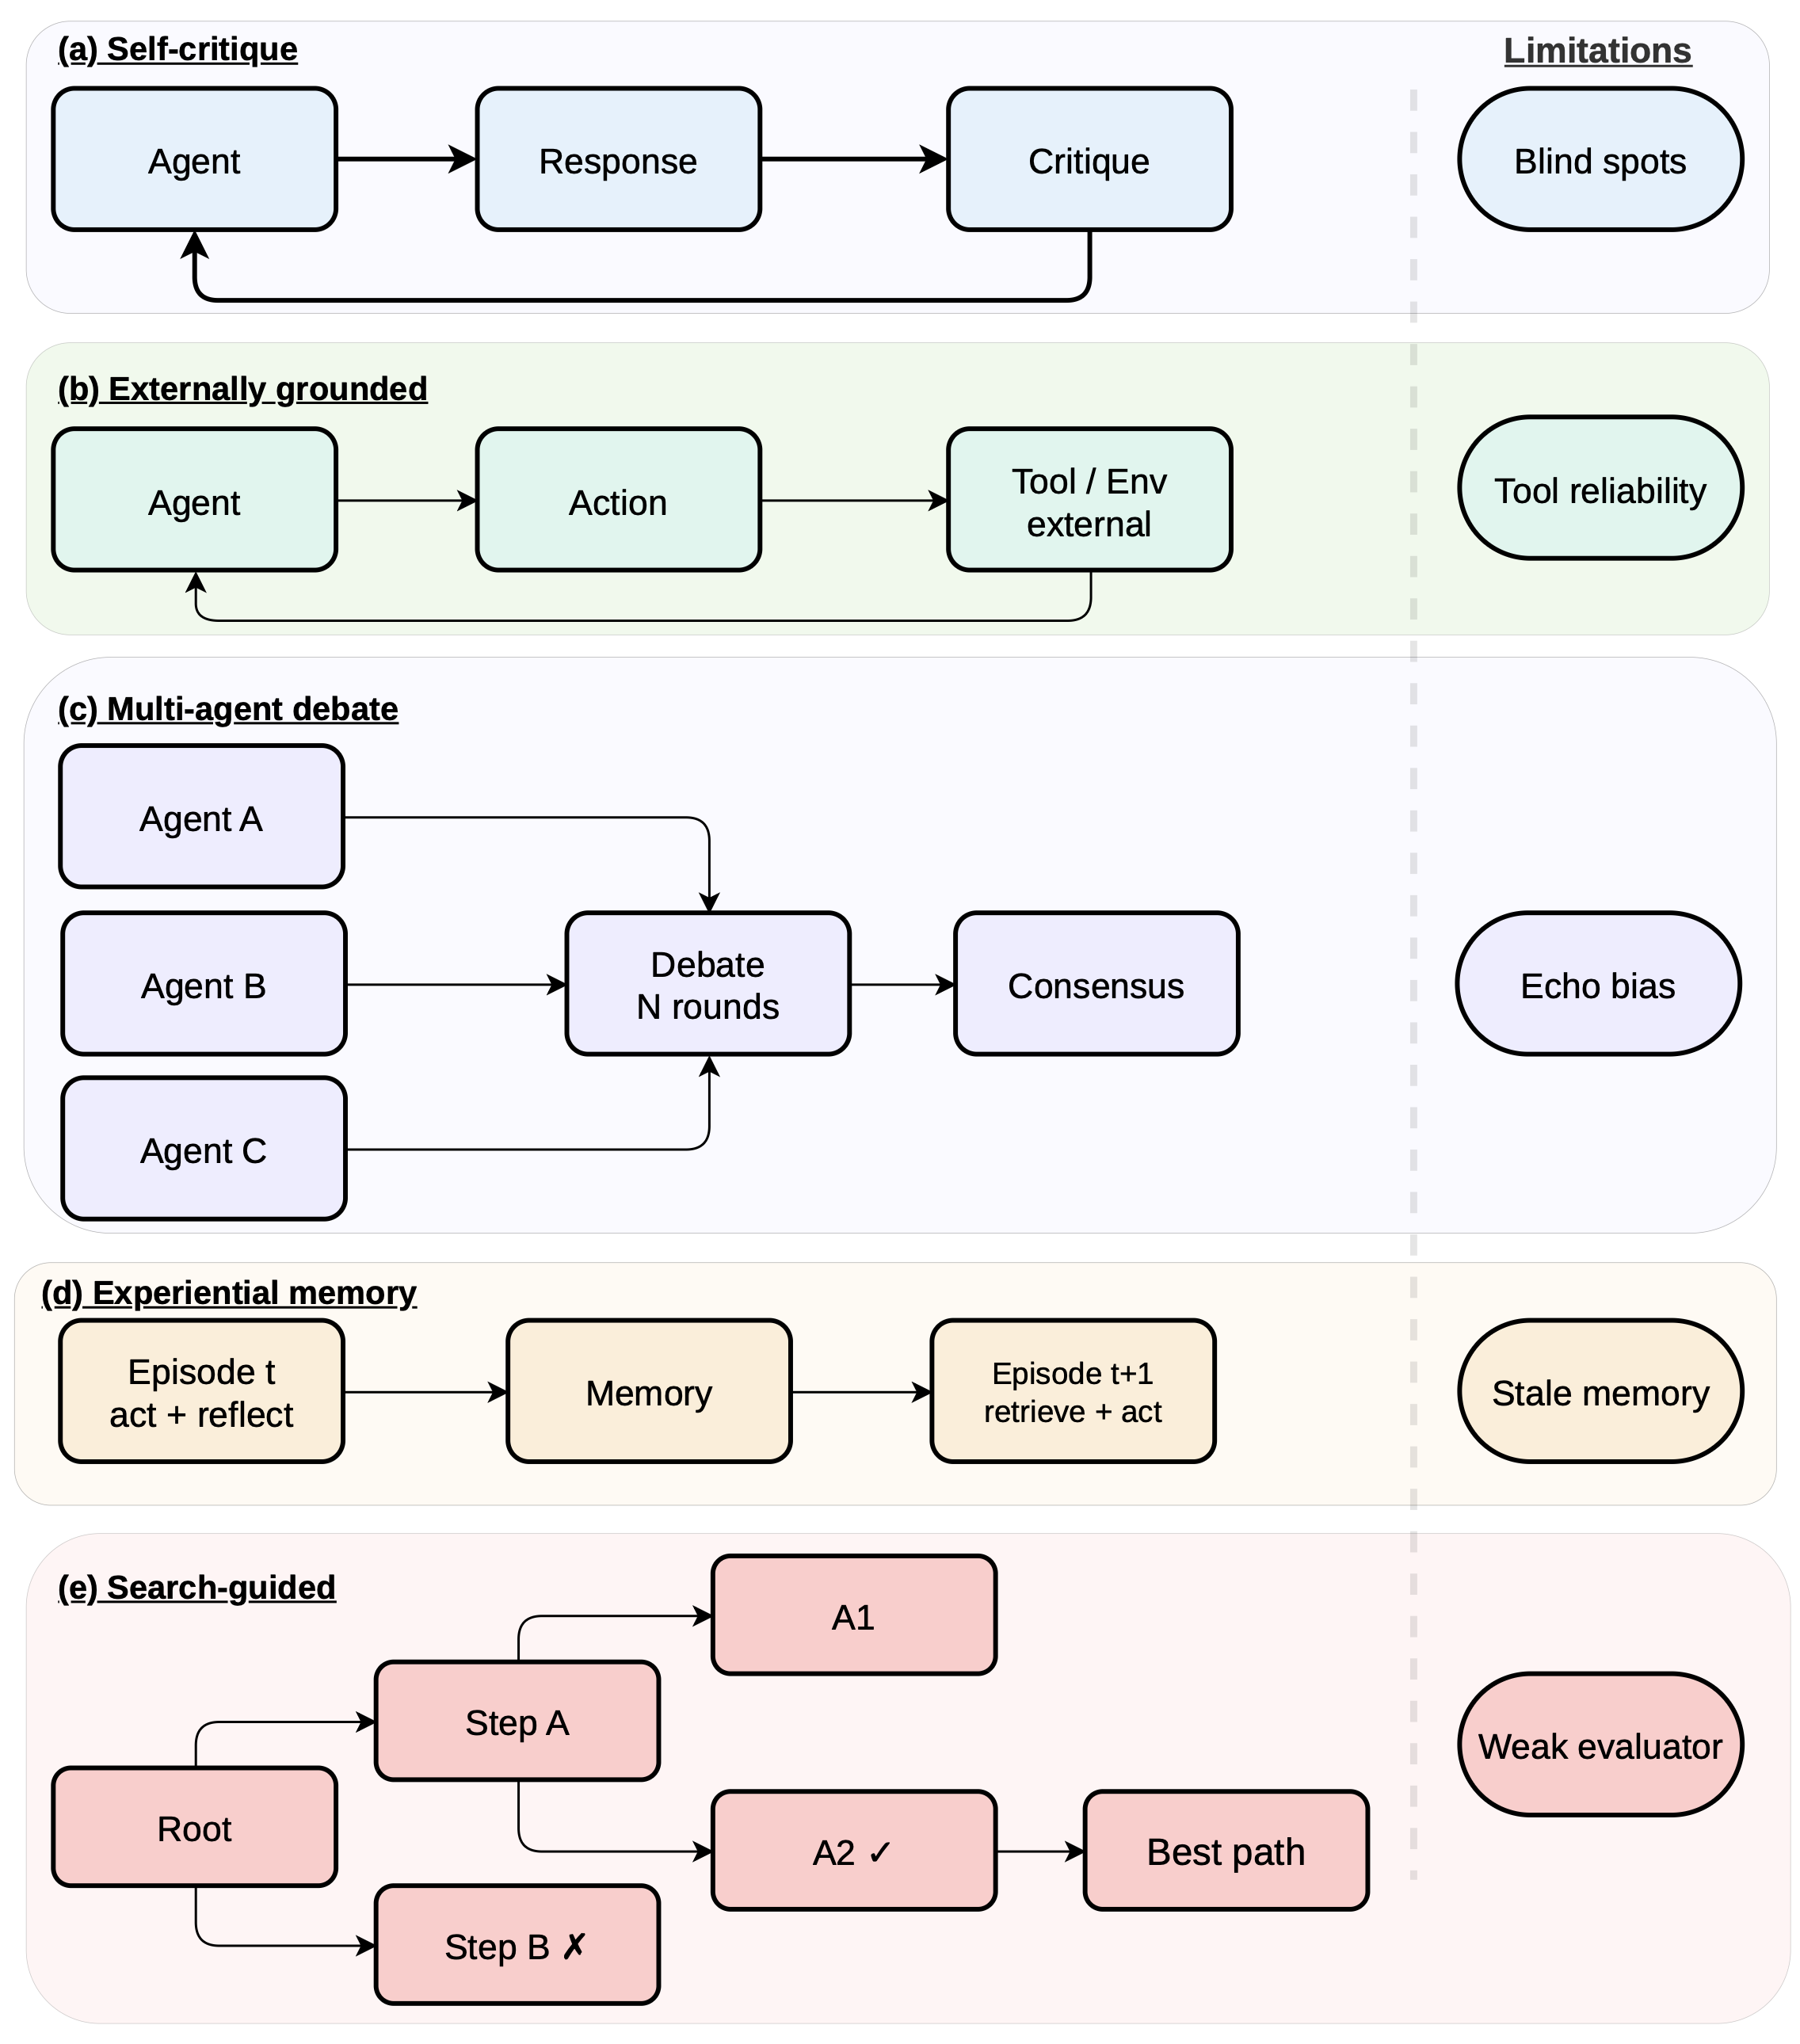
\includegraphics[width=\linewidth]{paper_images/Figure-3-new.png}
    \Description{Five panels depict self-critique, externally grounded critique, multi-agent debate, experiential memory, and evaluator feedback in search. A limitations column identifies blind spots, tool reliability, echo bias, stale memory, and weak evaluation.}
    \caption{Inference-time verbal feedback mechanisms: self-critique, externally grounded critique, multi-agent debate, experiential memory, and evaluator feedback in search.}
    \label{supp:fig:inference-time}
\end{figure}

\subsubsection{Self-critique and external grounding}
\label{supp:subsec:deliberative-critique}

Self-Refine formalized iterative self-critique and revision \citep{madaan2023selfrefine}, building on Constitutional AI's demonstration that written principles can guide revisions \citep{bai2022constitutional}. A separately trained critic improves reasoning relative to a shared generator-critic loop \citep{paul2024refiner}. Other evaluations show that self-correction degrades when the critique source shares the generator's failure modes \citep{huang2023large,kamoi2024can}, especially for smaller models \citep{olausson2024self}. Socratic decomposition creates independently checkable steps \citep{shi2025ssr}, and parallel refinement widens the candidate pool \citep{wang2025learning}, but neither supplies knowledge absent from the model.

External grounding anchors critique in deterministic evidence. Toolformer established the broader tool-use setting \citep{schick2023toolformer}; execution traces, tests, search results, and API responses then became reusable feedback sources \citep{chen2024teaching,gou2024toratoolintegratedreasoningagent}. CRITIC, SWE-agent, and executable-code agents use such evidence to produce corrected outputs \citep{gou2024critic,yang2024swe,wang2024executable}. Reinforcement learning can train a model to exploit the same feedback more effectively \citep{gehring2024rlef}. The system cost shifts from critic circularity to infrastructure, latency, and correct interpretation of the external trace.

\subsubsection{Debate systems and oversight evidence}
\label{supp:subsec:deliberative-debate}

Multi-agent debate assigns parallel model instances distinct perspectives or roles \citep{hong2024metagpt}. Identical models can improve through critique exchange \citep{du2023debate}, role diversity can strengthen evaluation \citep{chan2023chatevalbetterllmbasedevaluators}, and models can be trained to revise under conflicting opinions \citep{liu2026learningselfdebatepreparingreasoning}. Adaptive heterogeneous groups also improve mathematical reasoning \citep{zhou2025adaptive}.

The economic evidence is mixed. Debate provides limited gains over single-agent scaling on mathematical reasoning but becomes more useful as task difficulty rises and base capability falls; on safety tasks, collaborative refinement can increase vulnerability while diverse groups reduce attack success \citep{yang2025revisiting}. A broader evaluation across debate methods, benchmarks, and foundation models finds that debate often fails to beat chain-of-thought or self-consistency despite substantially higher inference cost, with model heterogeneity the most reliable intervention \citep{zhang2025stop}. Shared biases produce redundant consensus \citep{estornell2024multi,liang2024encouragingdivergentthinkinglarge}, and simpler single-agent strategies remain competitive \citep{choi2026debate}.

Communication topology controls part of that cost. Full broadcast incurs substantial token overhead \citep{choi2026debate}; sparse connections reduce it \citep{li2024improving}. Other methods retain only maximally disagreeing responses per round \citep{nguyen2026hear} or ask agents to express confidence so a knowledgeable minority does not capitulate to the group \citep{lin2025enhancing}.

Debate also serves scalable oversight. It raises weaker model and human judge accuracy above naive baselines \citep{khan2024debating}, and it can outperform consultancy under information asymmetry \citep{kenton2024scalable}. When transcripts become training data, rewards, or distilled weights, the same mechanism moves from deliberation to learning \citep{motwani2024malt,subramaniam2025multiagent,park2025maporl,yi2026latent}.

\subsubsection{Experiential-memory systems}
\label{supp:subsec:deliberative-memory}

Dedicated surveys catalog episodic, semantic, and procedural memory stores \citep{zhang2025survey,du2026memory}. The narrower VRL question is whether a stored linguistic artifact is consumed as feedback in a later context. Deployment-time learning has also been proposed as a lifecycle stage after pretraining and post-training \citep{guo2026cascade}.

Raw reflections are inexpensive and fit closely recurring tasks. Reflexion reports a HumanEval pass@1 of 91 percent through stored self-reflection \citep{shinn2023reflexion}. When experience must transfer, distilled principles remove episode-specific detail. ExpeL contrasts successes and failures; MetaReflection compresses failed trials; related systems induce reusable workflows or strategy notes \citep{zhao2024expel,gupta2024metareflection,wang2024agent,ouyang2025reasoningbank,suzgun2026dynamic}. Structured stores become useful when scale or collaboration makes flat retrieval expensive. Interlinked notes, consolidation, team graphs, and reconstruction-time retrieval trade management overhead for selective access \citep{xu2025amem,chhikara2025mem0,zhang2025gmemory,ji2026memory}. Tasks requiring reliable re-execution favor code and instruction libraries whose skills can be tested and admitted with evidence \citep{wang2023voyager,fang2025memp,zhang2026agentfactory,lin2026museautoskill,zhou2026mementoskills,yang2026autoskill,liu2026skillsvote}.

Writing policy is a second design axis. Append-only stores suit short, stationary deployments. Longer-lived agents need utility-based pruning \citep{cao2025remember,zhang2026liveevo}. Memory-R1, AutoMem, and SkillRL train add, update, delete, or no-op decisions \citep{yan2025memoryr1,wu2026automem,xia2026skillrl}. Meta-evolution searches the entire encode, store, retrieve, and manage pipeline \citep{zhang2025memevolve,liu2026mempro,zhang2026memskill}. These writers can be trained by scalar outcomes while their stored text still acts through the context window.

Persistence amplifies both value and error. Large stores complicate retrieval \citep{park2023genagents}; stale knowledge misleads in changing environments \citep{zhang2025survey}; and injected memories cause cross-session drift \citep{dong2026memory}. Forced consolidation can itself corrupt evidence, with raw-episode retention outperforming continual summarization in one controlled study \citep{zhang2026useful}. Memory evaluation increasingly probes retrieval, test-time learning, long-range understanding, and selective forgetting \citep{tan2025membench,hu2025evaluating,wei2025evomemory,belikova2026managing}.

\subsubsection{Evaluator feedback in search}
\label{supp:subsec:deliberative-search}

Search systems explore several candidate paths and use language to select which to expand or prune \citep{wang-etal-2025-dont}. Tree of Thoughts adds self-evaluation to a tree over intermediate thoughts \citep{wei2022chain,yao2023tree}; Reasoning via Planning and Graph of Thoughts generalize the topology and permit aggregation or refinement across branches \citep{hao2023reasoning,besta2024graph}. Node-level verbal evaluation can terminate bad paths early, but repeated evaluation multiplies model calls relative to single-pass generation \citep{xie2023self}. This catalog excludes search procedures whose selection signal contains no language, including majority voting over sampled chains.

\subsection{Extended Catalog: Language as Learning Signal}
\label{supp:sec:learning}

\subsubsection{Feedback-conditioned and self-improvement systems}
\label{supp:subsec:learning-conditioned}

Feedback-conditioned modeling trains on triples containing an input, critique, and revised output. Early methods discarded the critique after using it to produce the target \citep{scheurer2023training,chen2024ilf}. ALT retains it as conditioning context \citep{lloret2024towards}, while the feedback-conditional policy learns the response posterior given feedback and adds an online positive-feedback bootstrapping stage \citep{luo2025fcp}. Critique use can itself be trained: didactic multi-turn interactions teach a smaller model to predict and incorporate teacher feedback \citep{klissarov2026improving}. RLVF scopes a verbal instruction by generating preference data that mark where it should and should not apply \citep{stephan2024rlvf}. The corresponding risk is over-receptiveness, since models can learn to follow incorrect critiques \citep{sharma2024towards}.

Self-improvement uses feedback to select generated data \citep{singh2023beyond}. Filters include final-answer correctness in STaR \citep{zelikman2022star}, constitutional compliance \citep{bai2022constitutional}, majority agreement \citep{huang2022selfimprove}, and a model's own iterated judgment \citep{yuan2024self}. Generator-judge coupling can amplify systematic bias over rounds \citep{shumailov2023curse}. Multiagent finetuning preserves diverse reasoning by training a society of models on interaction data \citep{subramaniam2025multiagent}. Agent-R replaces whole-trajectory selection with targeted recovery, using tree search to connect failed paths to adjacent successful ones \citep{yuan2025agentr}.

\subsubsection{Trained critics}
\label{supp:subsec:learning-critics}

Critics obtain supervision from several sources. MultiCritique distills feedback from several agents into fine-tuning and preference data \citep{lan2024training}. CTRL trains a critic to maximize the correction performance of a fixed code generator \citep{xie2025teaching}. Critique-RL separates discriminability from helpfulness by first reinforcing rule-based error detection and then adding refinement reward \citep{xi2025critiquerl}. DeepCritic combines long-form critique training with reinforcement over human or Monte Carlo step labels \citep{yang2025deepcritic}, while AutoMathCritique trains an actor-critic pair on automatically generated step feedback \citep{xi2024enhancing}. Critique-guided improvement jointly trains a critic and an actor so feedback steers exploration rather than only ranking final responses \citep{yang2025lighthouse}. These systems show why feedback quality must be measured by both error localization and the correction it induces.

\subsubsection{Multi-agent and self-play training}
\label{supp:subsec:learning-multiagent}

MALT samples role-specific search trees for a generator, verifier, and refiner, then propagates outcome rewards to each role through value iteration \citep{motwani2024malt}. MAPoRL co-trains participants against correctness and collaboration incentives \citep{park2025maporl}. Self-play removes external annotation through adversarial word games \citep{cheng2024selfplaying}, games a model plays against itself \citep{kuba2025language}, or proposer, solver, and judge roles instantiated from one model \citep{chen2025multiagent}. SPC evolves a critic against a generator trained to produce difficult-to-detect reasoning errors \citep{chen2025spc}.

The communication channel can itself receive reward. Influence-based rewards elicit accusation and evidence-giving in social deduction \citep{sarkar2025training}, while dialogue-game environments use interactive group-relative optimization \citep{horst2025playpen}. Persuasion-balanced training prevents debaters from learning to reject beneficial persuasion along with adversarial persuasion \citep{stengeleskin2024teaching}. Explicit debate can also be internalized: latent agents distill transcripts into a single model \citep{yi2026latent}. Related oversight systems reward prover checkability \citep{kirchner2024prover}, use debate outcomes in sequential decision making \citep{sukovic2024reward}, train debaters through self-play \citep{arnesen2024training}, or use debate for weak-to-strong supervision \citep{lang2025debate}.

\subsubsection{Process supervision and preference shaping}
\label{supp:subsec:learning-process}

The canonical process-supervision dataset uses positive, negative, or neutral click labels for individual reasoning steps \citep{lightman2024let}. Such labels are scalar, but generative PRMs consume language before scoring \citep{zhao2025genprm,liu2025agenticreinforcementlearningimplicit}. Step-level critique also qualifies when downstream machinery converts its content into credit. Process feedback improves localization relative to outcome-only labels \citep{lightman2024let,uesato2022solving}, and the cost of manual step annotation motivated automatic labeling with Math-Shepherd and OmegaPRM \citep{wang2024mathshepherd,luo2024improve}. Its practical limits remain expensive verification and difficulty defining a locally correct step outside mathematics and code.

Preference shaping is the maximally compressed endpoint. Preference-based reinforcement learning supplies the lineage \citep{christiano2017deep}; InstructGPT trains a reward model and optimizes it with proximal policy optimization \citep{ouyang2022training,schulman2017proximal,stiennon2020learning}; and DPO removes the explicit reward model \citep{rafailov2023direct}. KTO, ORPO, SimPO, and related objectives modify the implicit preference loss \citep{ethayarajh2024kto,hong2024orpo,meng2024simpo,azar2024general}, while RLAIF replaces human labels with model judgments \citep{lee2023rlaif}. Online optimization queries fresh policy samples, fixed offline datasets inherit coverage gaps, and iterated preference collection occupies the middle ground \citep{yuan2024self}. Open problems for this scalar endpoint are surveyed separately \citep{casper2023open}.

Across the compression spectrum, quantitative evidence is method-specific rather than directly comparable. GOLF reports improved sample efficiency by injecting group-level critiques into sparse-reward regions \citep{huang2026bootstrapping}; Text2Grad converts free-form critiques into span-level rewards \citep{wang2026text2gradreinforcementlearningnatural}. These results motivate controlled comparisons that hold model, data, feedback budget, and verifier strength fixed.

\subsection{Extended Catalog: The Verbal Reward Stack}
\label{supp:sec:reward-stack}

\subsubsection{Verifiable outcomes and rubric supply}
\label{supp:subsec:reward-verifiable-rubric}

Tulu 3 combines supervised fine-tuning, preference optimization, and reinforcement learning against programmatic checks in an open post-training pipeline \citep{lambert2024tulu}. DeepSeek-R1 reports emergent reflection and verification under outcome-only reinforcement learning \citep{guo2025deepseek}. Verifiable rewards remain sparse and domain-limited. Agent-RLVR adds teacher-style plans and error feedback to failed software-engineering attempts, then trains a reward model on the guided data \citep{da2025agentrlvr}. Budget mismatches, attempt inflation, calibration drift, and benchmark contamination can confound headline RLVR gains \citep{wu2025position}.

Rubric rewards replace a ground-truth check with instance-specific criteria. Rubrics as Rewards reports gains over direct Likert-style judging in health and reasoning tasks \citep{gunjal2025rubrics}; checklist feedback improves hard instruction satisfaction \citep{viswanathan2025checklists}. Static banks support broad, stable task distributions, with human, synthetic, coarse-to-fine, or contrastively generated criteria \citep{huang2025reinforcement,li2026rubrichub,liu2025openrubrics}. Dynamic rubrics adapt to the current policy or case mix through online generation, policy-coupled evolution, self-rewarding, or case-conditioned criteria \citep{rezaei2025online,guan2026evorubric,ye2025selfrewarding,wang2025infimedorbit}. Selective verification invokes external checks only for likely violations \citep{wu2025rlac}; process-oriented rubrics detect invalid derivations that final-answer checks miss \citep{yuan2025curing}. Prior work also surveys rubrics across evaluation, training, and safety \citep{chen2026from}.

\subsubsection{Generative reward models}
\label{supp:subsec:reward-generative}

Generative verifiers cast reward modeling as next-token prediction and write a verification rationale before the verdict \citep{zhang2025genrm}. DeepSeek-GRM trains principle generation and critique, then allocates inference-time samples with a meta reward model \citep{liu2025inferencetime}. Related systems generate rubrics or reference solutions before judging \citep{chen2025rmr1}, spend adaptive compute on hard decisions \citep{guo2025reward}, turn judgment into a verifiable-reward task \citep{whitehouse2025j1}, or separate evaluation planning from execution \citep{saha2025learning}. Other variants optimize judgment traces with offline or online reinforcement learning \citep{huang2025thinkj}, extend judges to long-horizon reasoning \citep{hong2025thinkrm}, or pair a reasoning reward model with a dedicated benchmark \citep{zhou2025libra}.

Judge supervision is increasingly self-generated. Self-taught evaluators iterate without human preference labels \citep{wang2024selftaught}; joint critique and scalar prediction improves reward accuracy \citep{yu2024selfgenerated}; self-training produces reward models that emit labels with rationales \citep{wang2025gramr2}; and meta-rewarding asks the model to judge its own judgments \citep{wu2024metarewarding}. The explanation is not automatically trustworthy. Outcome-only training can produce correct verdicts supported by unsound critiques, while explicit critique supervision improves reliability \citep{wang2026reward}.

\subsubsection{Process reward models}
\label{supp:subsec:reward-process}

Human step annotation established the PRM lineage \citep{lightman2024let}. Math-Shepherd automates labels and applies stepwise policy optimization \citep{wang2024mathshepherd}; OmegaPRM uses divide-and-conquer search to locate the first error and build a large step-level dataset \citep{luo2024improve}. ProcessBench finds weak generalization beyond common mathematics benchmarks and cases where prompted critics outperform trained PRMs \citep{zheng2024processbench}. A companion analysis shows that Monte Carlo labels can underperform judge or human annotations, that best-of-N evaluation drifts toward outcome scoring, and that consensus filtering improves label quality \citep{zhang2025lessons}.

Generative PRMs join step verification with language reasoning. ThinkPRM generates a verification chain for every step \citep{khalifa2025processrewardmodelsthink}; StepWiser trains stepwise reasoning with reinforcement from rollout outcomes \citep{xiong2025stepwiser}; and DG-PRM selects fine-grained criteria dynamically per step \citep{yin2025dynamic}. SPARK synthesizes verification data for domains without directly checkable answers \citep{rahman2025spark}, and related pipelines extend automatic step annotation to multimodal reasoning \citep{du2025mmprm}. Response-level rubrics can also be converted to token-level credit through a relevance discriminator \citep{xu2026rubrics}.

\subsubsection{Boundary failures and defenses}
\label{supp:subsec:reward-boundary}

The scalarization boundary creates exploitable slack at every rung. Outcome-only optimization can encourage invalid ``Miracle Steps'' \citep{yuan2025curing}; static rubrics become stale or omit failure modes \citep{rezaei2025online}; and rubric-based verifiers can prefer a trained checkpoint even when rubric-free judges prefer the base model \citep{mahmoud2026reward}. Generative judges can reach correct verdicts from unsound critiques \citep{wang2026reward}, and misestimated step labels corrupt PRM training \citep{zhang2025lessons}. RLVR results can also shrink under budget-matched evaluation \citep{wu2025position}.

Proposed defenses operate at the same boundary: cross-family judge panels and verifier-free diagnostics \citep{mahmoud2026reward}, peer consensus over evolving rubrics \citep{guan2026evorubric}, format constraints on PRM-driven reinforcement learning \citep{rahman2025spark}, and consensus filtering of step labels \citep{zhang2025lessons}. These methods reduce known failures but do not remove the information lost when critique text becomes a scalar.
